\begin{problem}
试结合WSDL文件的结构,说明WSDL文档记载了哪些服务的哪些信息,并阐述为何需要将WSDL文件分为抽象部分和具体部分。
\end{problem}

\begin{solution}
\begin{figure}[H]
    \vspace{-0.5em}
	\centering
	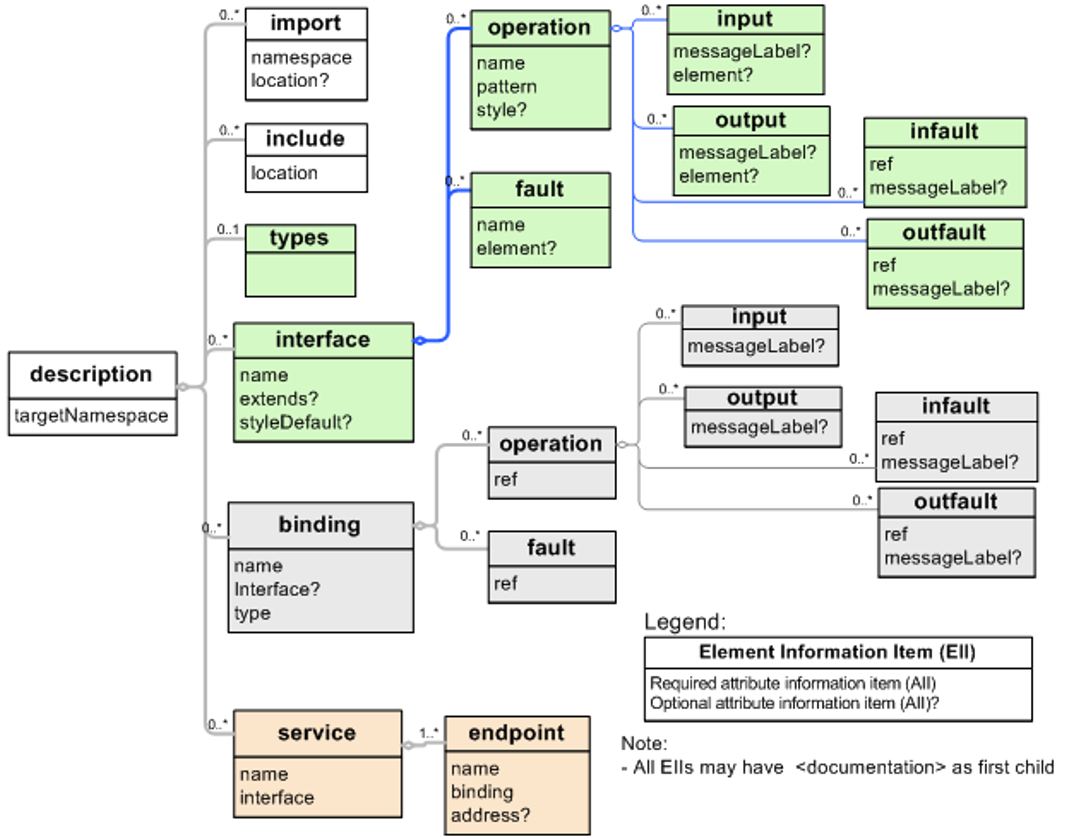
\includegraphics[width=0.68\textwidth]{WSDL 2.0信息集结构.png}
    \vspace{-1em}
\end{figure}

\vspace{-0.5em}
\begin{spacing}{1.2}
    \begin{longtable}{|m{4cm}|m{9cm}|}
        \hline
        \multicolumn{1}{|c|}{WSDL回答了}  &  \multicolumn{1}{c|}{WSDL提供了}\\ \hline
        \vspace{-1.3em}
        \begin{itemize}[leftmargin=1.5em,itemsep=-2pt]
            \item 服务用来干什么
            \item 服务在哪
            \item 如何调用服务
            \vspace{-1.5em}
        \end{itemize} &  
        \vspace{-1.3em}
        \begin{itemize}[leftmargin=1.5em,itemsep=-2pt]
            \item 功能信息(调用某一个特定的操作,这个操作能被用来完成面向服务的一项功能)
            \item 消息结构(如何说明消息交互中的数据类型)
            \item 协议绑定(如何将抽象消息映射为具体的网络传输)
            \vspace{-1.5em}
        \end{itemize}
        \\\hline
    \end{longtable}
\end{spacing}
\vspace{-1em}

\begin{spacing}{1.2}
    \begin{longtable}{|m{8.5cm}|m{6.5cm}|}
        \hline
        \multicolumn{1}{|c|}{\textbf{抽象部分}} & \multicolumn{1}{c|}{\textbf{具体部分}} \\ \hline
        \vspace{-1.3em}
        \begin{itemize}[leftmargin=1.5em,itemsep=-3pt]
            \item Types:独立于机器和语言的类型定义
            \item Message:通信消息的数据结构的抽象类型化定义。使用Types所定义的类型来定义整个消息的数据结构。  
            \item Operation:对服务中所支持的操作的抽象描述,一般单个Operation描述了一个访问入口的请求/响应消息对。
            \item Interface:对于某个访问入口点类型所支持的操作的抽象集合,这些操作可以由一个或多个服务访问点来支持。
        \vspace{-1.5em}
        \end{itemize}                                           
            & 
        \vspace{-1.3em}
        \begin{itemize}[leftmargin=1.5em,itemsep=-3pt]
            \item Binding:特定端口类型的具体协议和数据格式规范的绑定。
            \item Endpoint:定义为协议/数据格式绑定与具体Web访问地址组合的单个服务访问点。
            \item Service:相关服务访问点的集合。
        \vspace{-1.5em}
        \end{itemize}  
        \\ \hline
    \end{longtable}
    \vspace{-1em}
\end{spacing}

WSDL简化结构
\begin{figure}[H]
    \vspace{-0.7em}
	\centering
	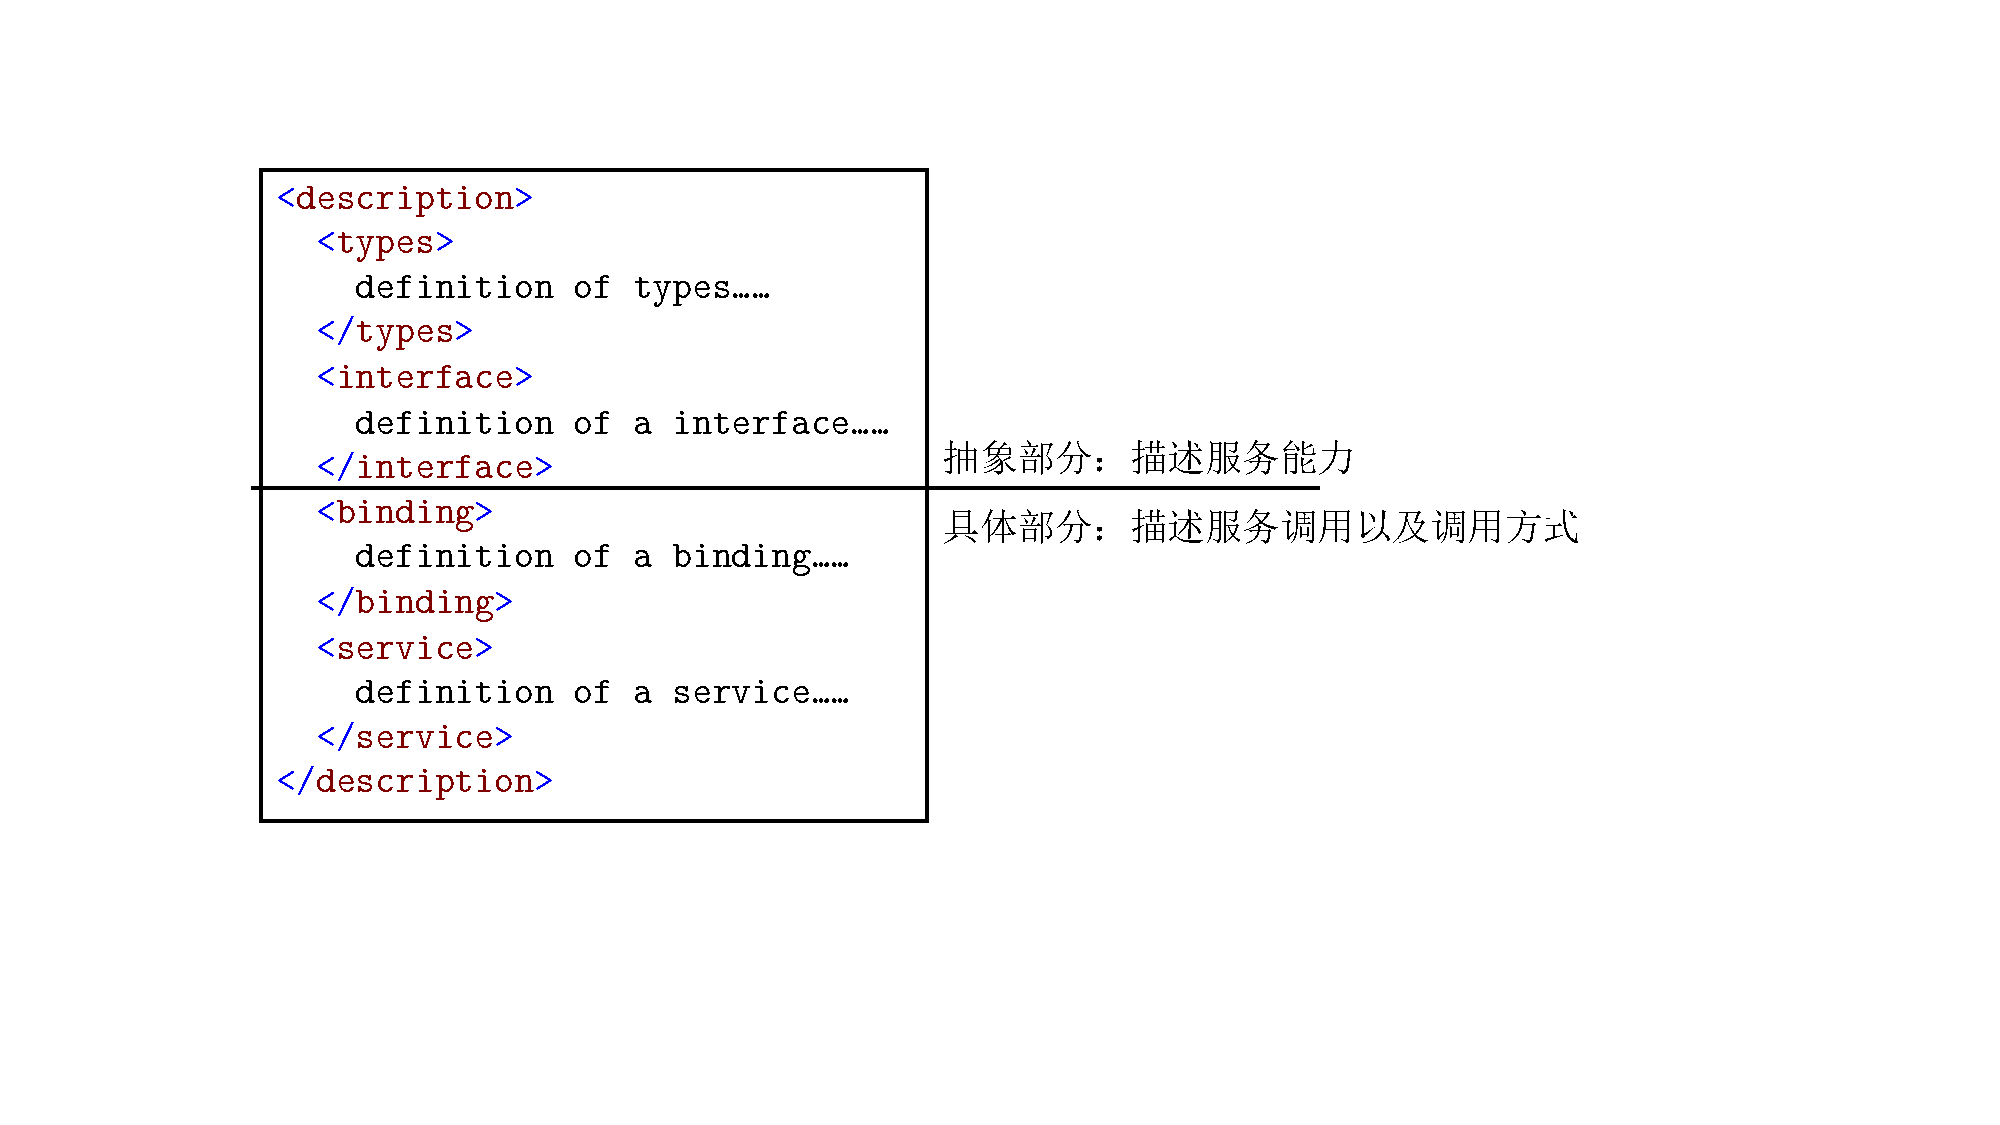
\includegraphics[width=0.7\textwidth]{WSDL简化结构.pdf}
    \vspace{-1em}
\end{figure}

将WSDL文件分为抽象部分和具体部分:
\begin{itemize}
    \item 抽象部分以独立于平台和语言的方式定义服务的逻辑意义,并不包含任何随机器或语言而变的元素,使不同的服务调用者都能调用实现;具体部分则包含了随网站而异的东西,由各实现方依据自己的情况定制。将二者分离能在保证可复用的同时又不局限各实现的个性化定制,同时使得Web服务的接口和实现分离,使得Web服务的接口更加通用和可重用,便于Web服务的维护和扩展,提高互操作性。
    \item 定义服务与实现服务可能是不同的部门或者组织,那么抽象部分与具体部分的WSDL也应当由各自的部门定义、持有与管理。
\end{itemize}

\end{solution}